\documentclass{zc-ust-hw}

\usepackage{circuitikz}

\name{SalahDin Ahmed Salh Rezk}
\id{202201079}
\course{Electric Circuits (ENGR 210)}
\assignment{Final Project}

\begin{document}

\maketitle
\tableofcontents
\listoffigures
\listoftables
\lstlistoflistings
\begin{abstract}
  This report describes the design of two circuits, Circuit 1 and Circuit 2,
  that meet the requirements specified in the project description. The
  theoretical values of the output voltages of the two circuits are calculated
  and compared to the simulation results. The two circuits are then cascaded,
  and the theoretical value of the output voltage of the cascaded circuits is
  calculated and compared to the simulation results. The simulation show that
  the theoretical values are very close to the simulation results.
\end{abstract}

\section{Problem Statements}
\label{sec:problem-statements}

Design two circuits, Circuit 1 and Circuit 2, that meet the following
requirements:

\begin{enumerate}
  \item Circuit 1 should have an output voltage, $V_{o1}$, equal to $K_a$ times
    the input voltage, $V_{i1}$.
  \item Circuit 2 should have an output voltage, $V_{o2}$, equal to $K_b$ times
    the input voltage, $V_{i2}$.
  \item The values of $K_a$ and $K_b$ can be found in a provided resource, and
    each circuit should use a different value for $K_a$ and $K_b$.
  \item The circuits should adhere to the following design constraints:
    \begin{enumerate}
      \item Resistors with resistance values ranging from 1KΩ to 10KΩ can be
        used.
      \item If an op-amp is used, only one op-amp is allowed.
      \item The circuits should be designed using the fewest components
        possible.
    \end{enumerate}
  \item Use the two circuits you have designed in part 1, cascade them.\\Is the
    equation $V_{o2} = K_a \cdot K_b \cdot V_{i1}$ satisfied?
    \begin{enumerate}
      \item Verify your answer using LTspice.
      \item Explain why the answer is 'YES' or 'NO'.
      \item If your answer is 'NO', redesign the circuit to meet the
        requirements in part 1 and satisfy the equation $V_{o2} = K_a \cdot K_b
        \cdot V_{i1}$.
    \end{enumerate}
\end{enumerate}

\section{Part 1}

\begin{table}[H]
  \caption{Circuit 1 and Circuit 2 parameters}\label{tab:1}
  \begin{center}
    \begin{tabular}{|c|c|c|c|}
      \hline
      $K_a$ & $K_b$ & $V_{i1}$ & $V_{i2}$ \\
      \hline
      2.4 & 0.65 & 1V & 1V \\
      \hline
    \end{tabular}
  \end{center}
\end{table}

Based on the requirements in Section~\ref{sec:problem-statements} and the
provided parameters in Table~\ref{tab:1}, the first circuit needs to have an
output voltage, $V_{o1}$, equal to 2.4 times the input voltage, $V_{i1}$, and
the second circuit needs to have an output voltage, $V_{o2}$, equal to 0.65
times the input voltage, $V_{i2}$. This means that the first circuit needs to
be an amplifier with a gain of 2.4, and the second circuit needs to be an
attenuator with a gain of 0.65.

\subsection{Circuit 1}
\label{sec:circuit-1}

As mentioned, the first circuit needs to be an amplifier with a gain of 2.4. To
achieve this, an operational amplifier (op-amp) is used. The op-amp is
configured in a non-inverting amplifier configuration. The gain of the
non-inverting amplifier is given by Equation~\ref{eq:1}.

\begin{equation}
  \label{eq:1}
  K_a = A_v = 1 + \frac{R_2}{R_1}
\end{equation}

The gain of the non-inverting amplifier is equal to the ratio of the feedback
resistor, $R_2$, and the input resistor, $R_1$, plus one. The feedback resistor
is connected between the output of the op-amp and the inverting input of the
op-amp. The input resistor is connected between the inverting input of the
op-amp and the input voltage, $V_{i1}$. The output voltage, $V_{o1}$, is
connected between the output of the op-amp and the inverting input of the
op-amp.

\begin{figure}[H]
  \centering
  \begin{circuitikz}[scale=0.85, transform shape]
    \draw (0,0) node[above]{$V_{i1}$} to[short, o-] ++(1,0)
    node[op amp, noinv input up, anchor=+](OA){}
    (OA.-) -- ++(0,-1) coordinate(FB)
    to[R=$R_1$] ++(0,-2) node[ground]{}
    (FB) to[R=$R_2$, *-] (FB -| OA.out) -- (OA.out)
    to [short, *-o] ++(1,0) node[above]{$V_{o1}$}
    ;
  \end{circuitikz}
  \caption{Non-inverting amplifier}
\end{figure}

Since the input voltage, $V_{i1}$, is 1V, the output voltage, $V_{o1}$, needs
to be 2.4V. The feedback resistor is chosen to be 1KΩ, and the input resistor
is chosen to be 1.4KΩ. The gain of the non-inverting amplifier is then shown in
Equation~\ref{eq:2}

\begin{equation}
  \label{eq:2}
  1 + \frac{1.4K\Omega}{1K\Omega} = 2.4
\end{equation}

However, the op-amp needs to be supplied with voltage. VCC is connected to the
positive supply voltage, and -VCC is connected to the negative supply voltage.
VCC is equal to 5V, and -VCC is equal to -5V. As the input voltage, $V_{i1}$,
is 1V, the output voltage, $V_{o1}$, will be 2.4V so 5V is enough to supply the
op-amp.

\subsection{Circuit 2}
\label{sec:circuit-2}

As mentioned, the second circuit needs to be an attenuator with a gain of 0.65.
To achieve this, a voltage divider is used. The voltage divider is made up of
two resistors, $R_1$ and $R_2$. The output voltage, $V_{o2}$, is connected
between the two resistors, and the input voltage, $V_{i2}$, is connected to one
of the resistors. The output of the voltage divider is given by
Equation~\ref{eq:3}.

\begin{equation}
  \label{eq:3}
  V_{o2} = V_{i2} \cdot \frac{R_2}{R_1 + R_2}
\end{equation}

It is possible, then, to rewrite the equation to solve for $R_2$ as shown in
Equation~\ref{eq:4}. The input voltage, $V_{i2}$, is 1V, and the output voltage,
$V_{o2}$, needs to be 0.65V. The value of $R_1$ is chosen to be 1KΩ, and the
value of $R_2$ is then calculated to be 1.857KΩ.

\begin{equation}
  \label{eq:4}
  R_2 = \frac{V_{o2} \cdot R_1}{V_{i2} - V_{o2}} = \frac{0.65 \cdot 1K\Omega}{1V - 0.65V} = 1.857K\Omega
\end{equation}

\begin{figure}[H]
  \centering
  \begin{circuitikz}[scale=0.85, transform shape]
    %Coordinates
    \coordinate (Earth) at (0,-1);
    \coordinate (A) at (0,0);
    \coordinate (B) at (0,3);
    \coordinate (C) at (6,3);
    \coordinate (D) at (6,0);
    % Circuit
    \draw (Earth) node[tlground]{} -- (A) to[V, v<=\( V_{i2} \)] (B) 
    to[R, l_=$R_1$, v^<, name=vr1] (C)
    to [R, l_=$R_2$, v^<, name=vr2, *-*] (D) -- (A);
    \draw (C) to[short, -o] ++(1,0) node[above]{$V_{o2}$};
  \end{circuitikz}
  \caption{Voltage divider}
\end{figure}


\subsection{LTspice Simulation}

The two circuits are simulated using LTspice. The simulation circuit is shown
in Figure~\ref{fig:ltspice-circuit}. The simulation results are shown in
Listing~\ref{lst:1}.

\begin{figure}[H]
  \begin{center}
    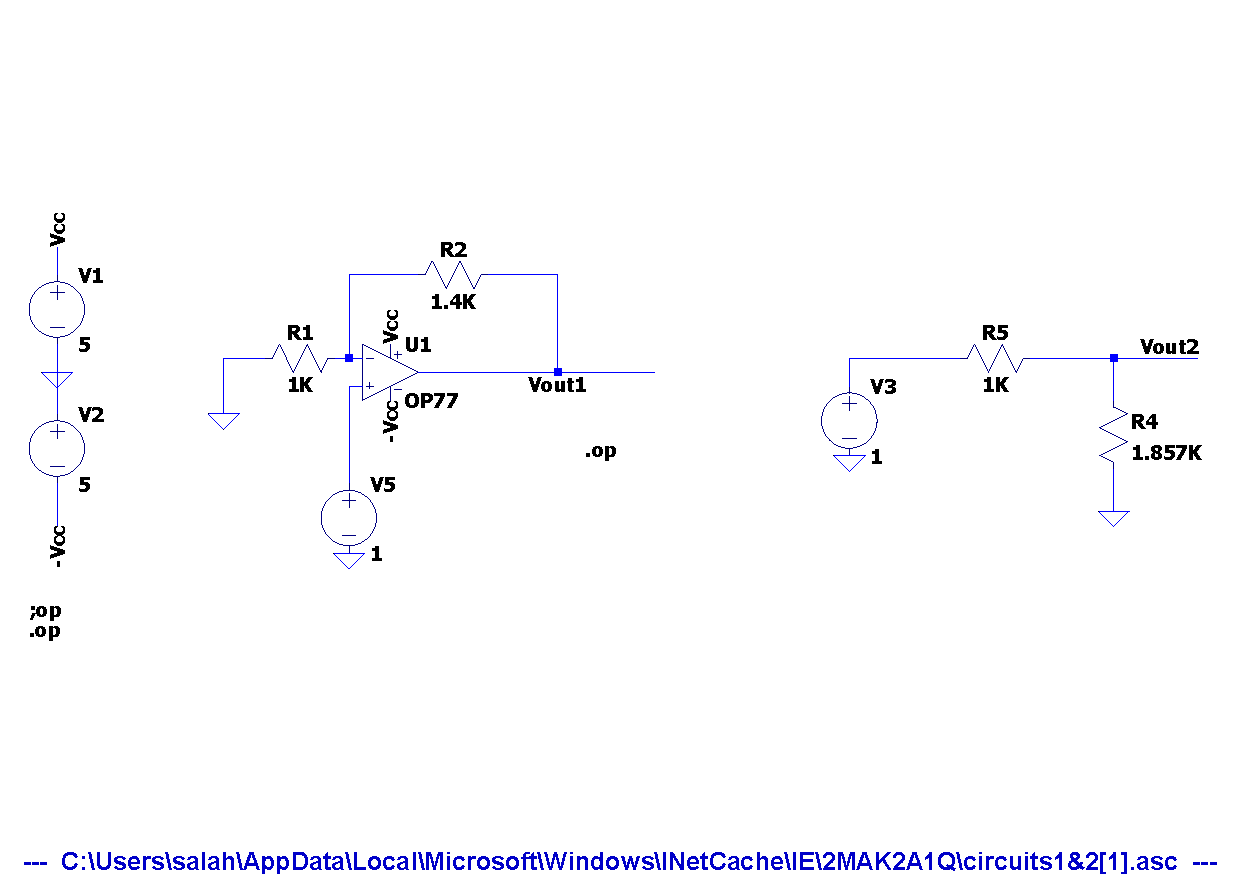
\includegraphics[width=0.85\textwidth]{figures/P1.pdf}
  \end{center}
  \caption{LTspice simulation results of the two circuits}\label{fig:ltspice-circuit}
\end{figure}

\begin{lstlisting}[caption=LTspice simulation results of the two circuits, label=lst:1]
       --- Operating Point ---

V(n001):	 1.00001	 voltage
V(n003):	 1	 voltage
V(vcc):	 5	 voltage
V(-vcc):	 -5	 voltage
V(vout1):	 2.40003	 voltage
V(vout2):	 0.649983	 voltage
V(n002):	 1	 voltage
I(R5):	 -0.000350018	 device_current
I(R4):	 0.000350018	 device_current
I(R2):	 0.00100001	 device_current
I(R1):	 0.00100001	 device_current
I(V3):	 -0.000350018	 device_current
I(V5):	 -1.34601e-009	 device_current
I(V2):	 -0.00075	 device_current
I(V1):	 -0.00175001	 device_current
Ix(u1:1):	 1.34601e-009	 subckt_current
Ix(u1:2):	 1.046e-009	 subckt_current
Ix(u1:99):	 0.00175001	 subckt_current
Ix(u1:50):	 -0.00075	 subckt_current
Ix(u1:39):	 -0.00100001	 subckt_current
\end{lstlisting}

From the simulation results, it can be seen that the output voltage, $V_{o1}$,
is 2.40003V and the output voltage, $V_{o2}$, is 0.649983V. These values are
very close to the theoretical values of 2.4V and 0.65V, respectively.
Table~\ref{tab:2} shows the simulation results.
 
\begin{table}[htpb]
  \caption{LTspice simulation results}\label{tab:2}
  \begin{center}
    \begin{tabular}[c]{|l|l|}
      \hline
      $V_{i1}$ & 1V \\
      \hline
      $V_{i2}$ & 1V \\
      \hline
      $V_{o1}$ & 2.40003V \\
      \hline
      $V_{o2}$ & 0.649983V \\
      \hline
    \end{tabular}
  \end{center}
\end{table}

\section{Part 2}

\subsection{Cascading the two circuits}

The output voltage, $V_{o1}$, is connected to the input voltage, $V_{i2}$, of
the second circuit. The output voltage, $V_{o2}$, is then measured. The
expected result is that the output voltage, $V_{o2}$, is equal to $K_a \cdot
K_b \cdot V_{i1}$, which is equal to 1.56V, as shown below.

\begin{align}
  V_{i 1} &= 1V \\
  V_{i2} = V_{o1} &= K_a \cdot V_{i1} \\
         &= 2.4 \cdot 1V = 2.4V \\
  V_{o2} &= V_{i 2} \cdot \frac{R_2}{R_1 + R_2} \\
         &= 2.4V \cdot \frac{1.857K\Omega}{1K\Omega + 1.857K\Omega} \\
         &= 1.56V
.\end{align}

\subsection{LTspice Simulation}

\begin{figure}[H]
  \begin{center}
    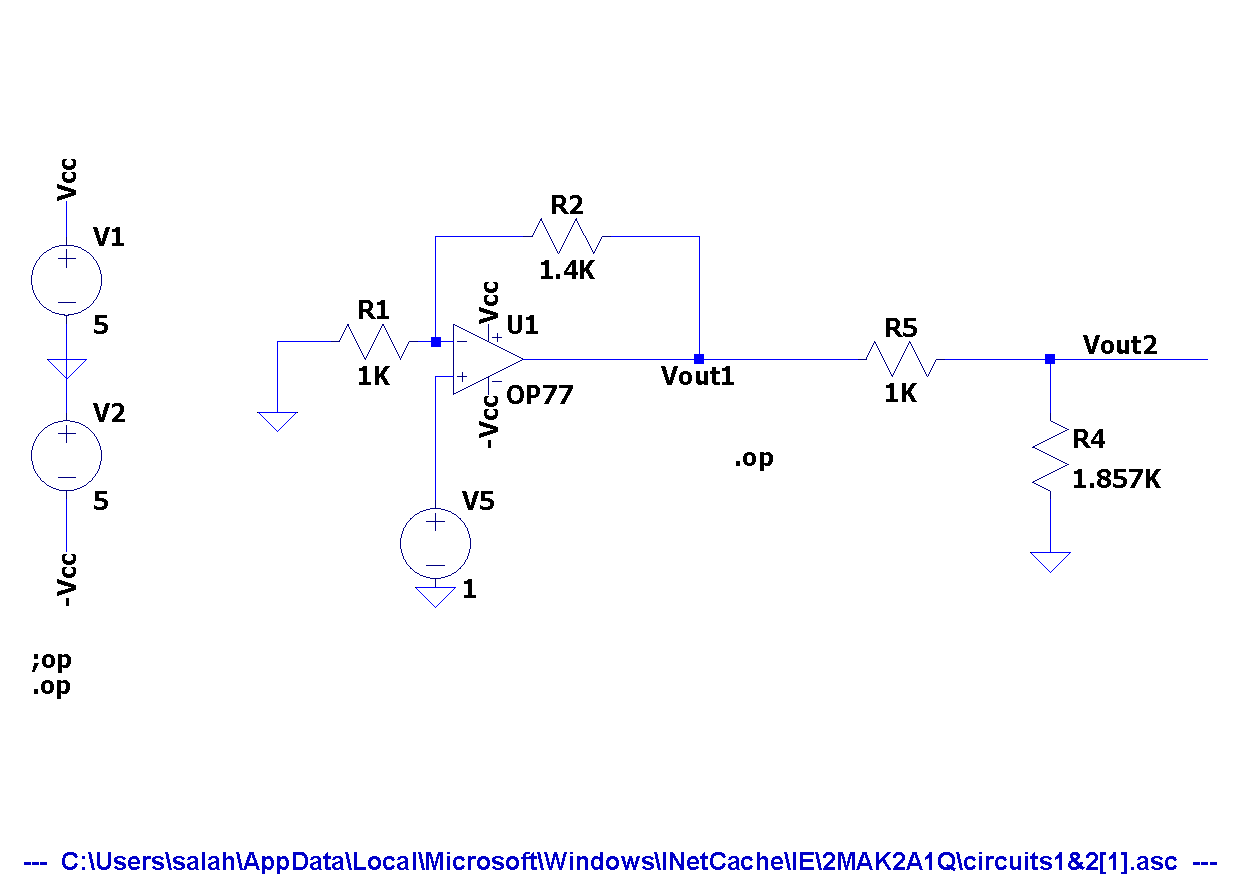
\includegraphics[width=0.85\textwidth]{figures/P2.pdf}
  \end{center}
  \caption{LTspice simulation results of the cascaded circuits}\label{fig:ltspice-circuit-2}
\end{figure}

\begin{lstlisting}[caption=LTspice simulation results of the cascaded circuits, label=lst:2]
       --- Operating Point ---

V(n001):	 1.00001	 voltage
V(n003):	 1	 voltage
V(vcc):	 5	 voltage
V(-vcc):	 -5	 voltage
V(vout):	 2.40003	 voltage
V(n002):	 1.55997	 voltage
I(R5):	 -0.000840051	 device_current
I(R4):	 0.000840051	 device_current
I(R2):	 0.00100001	 device_current
I(R1):	 0.00100001	 device_current
I(V5):	 -1.34601e-009	 device_current
I(V2):	 -0.00075	 device_current
I(V1):	 -0.00259006	 device_current
Ix(u1:1):	 1.34601e-009	 subckt_current
Ix(u1:2):	 1.046e-009	 subckt_current
Ix(u1:99):	 0.00259006	 subckt_current
Ix(u1:50):	 -0.00075	 subckt_current
Ix(u1:39):	 -0.00184006	 subckt_current
\end{lstlisting}

\newpage

From the simulation results, it can be seen that the output voltage, $V_{o1}$,
is 2.40003V and the output voltage, $V_{o2}$, is 1.55997V. These values are
very close to the theoretical values of 2.4V and 1.56V, respectively.
Table~\ref{tab:3} shows the simulation results. From these results, it can be
seen that the equation $V_{o2} = K_a \cdot K_b \cdot V_{i1}$ is satisfied.

\begin{table}[htpb]
  \caption{LTspice simulation results}\label{tab:3}
  \begin{center}
    \begin{tabular}[c]{|l|l|}
      \hline
      $V_{i1}$ & 1V \\
      \hline
      $V_{o1}$ & 2.40003V \\
      \hline
      $V_{o2}$ & 1.55997V \\
      \hline
    \end{tabular}
  \end{center}
\end{table}

\begin{equation}
  V_{o2} = K_a \cdot K_b \cdot V_{i1} = 2.4 \cdot 0.65 \cdot 1V = 1.56V
\end{equation}

\end{document}
